
We start with the standard traits that test primary and composite type categories (see Figure D.1).

\begin{tcolorbox}[colback=webgreen!5!white,colframe=webgreen!75!black]
\hspace*{0.75cm}Thanks to Howard Hinnant for providing this type hierarchy in \url{http://howardhinnant.github.io/TypeHiearchy.pdf}
\end{tcolorbox}

In general, each type belongs to exactly one primary type category (the white elements in Figure D.1). Composite type categories then merge primary type categories into higher-level concepts.

\begin{center}
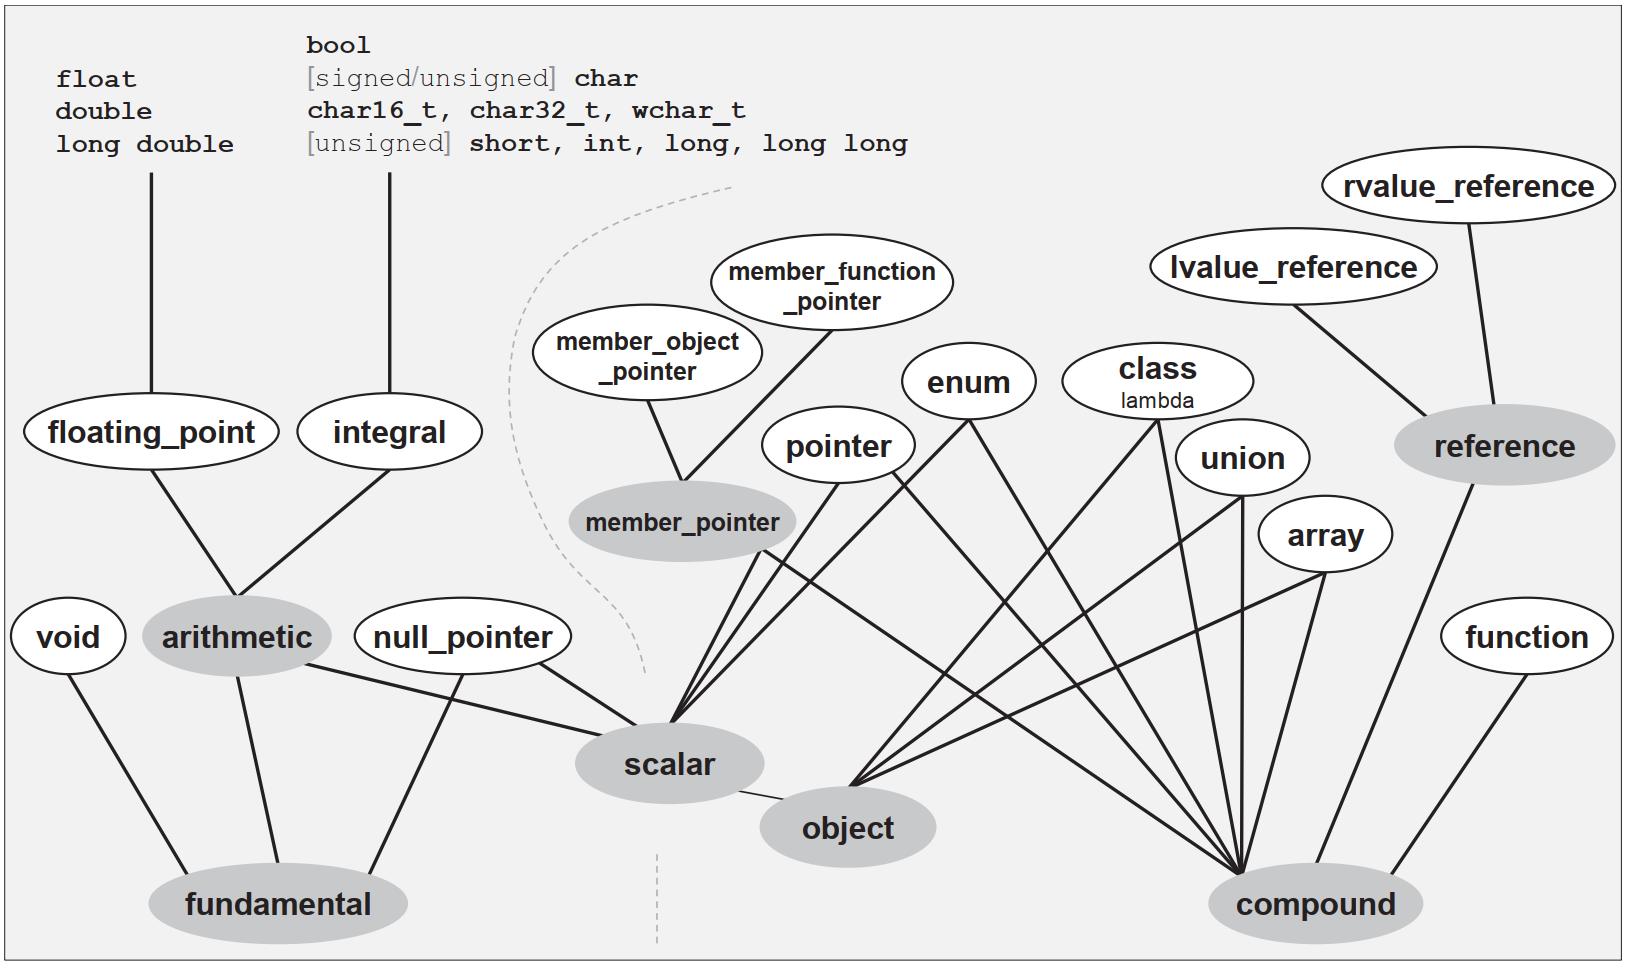
\includegraphics[width=0.8\textwidth]{content/Appendix/D/images/1.png} \\
Figure D.1. Primary and Composite Type Categories
\end{center}

\subsubsubsection{D.2.1\hspace{0.2cm}Testing for the Primary Type Category}

This section describes type utilities that test the primary type category of a given type. For any given type, exactly one of the primary type categories has a static value member that evaluates to true.

\begin{tcolorbox}[colback=webgreen!5!white,colframe=webgreen!75!black]
\hspace*{0.75cm}Before C++14, the only exception was the type of nullptr, std::nullptr\_t, for which all primary type category utilities yielded false, because is\_null\_pointer<> was not part of C++11.
\end{tcolorbox}

The result is independent of whether the type is qualified with const and/or volatile (cv-qualified).

Note that for types std::size\_t and std::ptrdiff\_t, is\_integral<> yields true. For type std::max\_align\_t, which one of these primary type categories yields true is an implementation detail (thus, it might be an integral or floating-point or class type). The language specifies that the type of a lambda expression is a class type (see Section 15.10.6 on page 310). Applying is\_class to that type therefore yields true.

\begin{table}[H]
	\begin{tabular}{|l|l|}
		\hline
		Trait                                                    & Effect                                                                                                         \\ \hline
		is\_void\textless{}T\textgreater{}                       & Type void                                                                                                      \\ \hline
		is\_integral\textless{}T \textgreater{}                  & \begin{tabular}[c]{@{}l@{}}Integral type (including bool, char, char16\_t, char32\_t,\\ wchar\_t)\end{tabular} \\ \hline
		is\_floating\_point\textless{}T \textgreater{}           & Floating-point type (float, double, long double)                                                               \\ \hline
		is\_array\textless{}T \textgreater{}                     & Ordinary array type (not type std::array)                                                                      \\ \hline
		is\_pointer\textless{}T \textgreater{}                   & \begin{tabular}[c]{@{}l@{}}Pointer type (including function pointer but not pointer to \\ nonstatic member)\end{tabular}                                  \\ \hline
		is\_null\_pointer\textless{}T \textgreater{}             & Type of nullptr (since C++14)                                                                                  \\ \hline
		is\_member\_object\_pointer\textless{}T \textgreater{}   & Pointer to a nonstatic data member                                                                             \\ \hline
		is\_member\_function\_pointer\textless{}T \textgreater{} & Pointer to a nonstatic member function                                                                         \\ \hline
		is\_lvalue\_reference\textless{}T \textgreater{}         & Lvalue reference                                                                                               \\ \hline
		is\_rvalue\_reference\textless{}T \textgreater{}         & Rvalue reference                                                                                               \\ \hline
		is\_enum\textless{}T \textgreater{}                      & Enumeration type                                                                                               \\ \hline
		is\_class\textless{}T \textgreater{}                     & Class/struct or lambda type but not a union type                                                               \\ \hline
		is\_union\textless{}T \textgreater{}                     & Union type                                                                                                     \\ \hline
		is\_function\textless{}T \textgreater{}                  & Function type                                                                                                  \\ \hline
	\end{tabular}
\end{table}

\begin{center}
Table D.1. Traits to Check the Primary Type Category
\end{center}

ype of a lambda expression is a class type (see Section 15.10.6 on page 310). Applying is\_class to that type therefore yields true.

std::is\_void < T >::value

\begin{itemize}
\item 
Yields true if type T is (cv-qualified) void.

\item 
For example:
\begin{lstlisting}[style=styleCXX]
is_void_v<void> // yields true
is_void_v<void const> // yields true
is_void_v<int> // yields false
void f();
is_void_v<decltype(f)> // yields false (f has function type)
is_void_v<decltype(f())> // yields true (return type of f() is void)
\end{lstlisting}

\end{itemize}

std::is\_integral < T >::value

\begin{itemize}
\item 
Yields true if type T is one of the following (cv-qualified) types:

\begin{itemize}
\item [-]
bool

\item [-]
 a character type (char, signed char, unsigned char, char16\_t, char32\_t, or wchar\_t)

\item [-]
an integer type (signed or unsigned variants of short, int, long, or long long; this includes std::size\_t and std::ptrdiff\_t)
\end{itemize}

\end{itemize}

std::is\_floating\_point < T >::value

\begin{itemize}
\item 
Yields true if type T is (cv-qualified) float, double, or long double
\end{itemize}

std::is\_array < T >::value

\begin{itemize}
\item 
Yields true if type T is a (cv-qualified) array type.

\item 
Recall that a parameter declared as an array (with or without length) by language rules really has a pointer type.

\item 
Note that class std::array<> is not an array type, but a class type.

\item 
For example:

\begin{lstlisting}[style=styleCXX]
is_array_v<int[]> // yields true
is_array_v<int[5]> // yields true
is_array_v<int*> // yields false

void foo(int a[], int b[5], int* c)
{
	is_array_v<decltype(a)> // yields false (a has type int*)
	is_array_v<decltype(b)> // yields false (b has type int*)
	is_array_v<decltype(c)> // yields false (c has type int*)
}
\end{lstlisting}

\item 
See Section 19.8.2 on page 453 for implementation details.

\end{itemize}

std::is\_pointer < T >::value
\begin{itemize}
\item 
Yields true if type T is a (cv-qualified) pointer. This includes:
\begin{itemize}
\item[-] 
pointers to static/global (member) functions

\item[-] 
parameters declared as arrays (with or without length) or function types
\end{itemize}

This does not include:

\begin{itemize}
\item[-] 
pointer-to-member types (e.g., the type of \&X::m where X is a class type and m is a nonstatic member function or a nonstatic data member)

\item[-] 
the type of nullptr, std::nullptr\_t
\end{itemize}

\item 
For example:

\begin{lstlisting}[style=styleCXX]
is_pointer_v<int> // yields false
is_pointer_v<int*> // yields true
is_pointer_v<int* const> // yields true
is_pointer_v<int*&> // yields false
is_pointer_v<decltype(nullptr)> // yields false

int* foo(int a[5], void(f)())
{
	is_pointer_v<decltype(a)> // yields true (a has type int*)
	is_pointer_v<decltype(f)> // yields true (f has type void(*)())
	is_pointer_v<decltype(foo)> // yields false
	is_pointer_v<decltype(&foo)> // yields true
	is_pointer_v<decltype(foo(a,f))> // yields true (for return type int*)
}
\end{lstlisting}

\item 
See Section 19.8.2 on page 451 for implementation details.
\end{itemize}

std::is\_null\_pointer < T >::value

\begin{itemize}
\item 
Yields true if type T is the (cv-qualified) std::nullptr\_t, which is the type of nullptr.

\item 
For example:
\begin{lstlisting}[style=styleCXX]
is_null_pointer_v<decltype(nullptr)> // yields true
void* p = nullptr;

is_null_pointer_v<decltype(p)> // yields false (p has not type std::nullptr_t)
\end{lstlisting}

\item 
Provided since C++14.
\end{itemize}

std::is\_member\_object\_pointer < T >::value

std::is\_member\_function\_pointer < T >::value

\begin{itemize}
\item 
Yields true if type T is a (cv-qualified) pointer-to-member type (e.g., int X::* or int (X::*)() for some class type X).
\end{itemize}

std::is\_lvalue\_reference < T >::value

std::is\_rvalue\_reference < T >::value

\begin{itemize}
\item 
Yields true if type T is a (cv-qualified) lvalue or rvalue reference type, respectively.

\item 
For example:
\begin{lstlisting}[style=styleCXX]
is_lvalue_reference_v<int> // yields false
is_lvalue_reference_v<int&> // yields true
is_lvalue_reference_v<int&&> // yields false
is_lvalue_reference_v<void> // yields false
is_rvalue_reference_v<int> // yields false
is_rvalue_reference_v<int&> // yields false
is_rvalue_reference_v<int&&> // yields true
is_rvalue_reference_v<void> // yields false
\end{lstlisting}

\item 
See Section 19.8.2 on page 452 for implementation details.
\end{itemize}

std::is\_enum < T >::value

\begin{itemize}
\item 
Yields true if type T is a (cv-qualified) enumeration type. This applies to both scoped and unscoped enumeration types.

\item 
See Section 19.8.5 on page 457 for implementation details.
\end{itemize}

std::is\_class < T >::value

\begin{itemize}
\item 
Yields true if type T is a (cv-qualified) class type declared with class or struct, including such a type generated from instantiating a class template. Note that the language guarantees that the type of a lambda expression is a class type (see Section 15.10.6 on page 310).

\item 
Yields false for unions, scoped enumeration type (despite being declared with enum class), std::nullptr\_t, and any other type.

\item 
For example:
\begin{lstlisting}[style=styleCXX]
is_class_v<int> // yields false
is_class_v<std::string> // yields true
is_class_v<std::string const> // yields true
is_class_v<std::string&> // yields false
auto l1 = []{};
is_class_v<decltype(l1)> // yields true (a lambda is a class object)
\end{lstlisting}

\item 
See Section 19.8.4 on page 456 for implementation details.
\end{itemize}

std::is\_union < T >::value

\begin{itemize}
\item 
Yields true if type T is a (cv-qualified) union, including a union generated from a class template that is a union template.
\end{itemize}

std::is\_function < T >::value

\begin{itemize}
\item 
Yields true if type T is a (cv-qualified) function type. Yields false for a function pointer type, the type of a lambda expression, and any other type.

\item 
Recall that a parameter declared as an function type by language rules really has a pointer type.

\item 
For example:
\begin{lstlisting}[style=styleCXX]
void foo(void(f)())
{
	is_function_v<decltype(f)> // yields false (f has type void(*)())
	is_function_v<decltype(foo)> // yields true
	is_function_v<decltype(&foo)> // yields false
	is_function_v<decltype(foo(f))> // yields false (for return type)
}
\end{lstlisting}

\item 
See Section 19.8.3 on page 454 for implementation details.
\end{itemize}

\subsubsubsection{D.2.2\hspace{0.2cm}Test for Composite Type Categories}

The following type utilities determine whether a type belongs to a more general type category that is the union of some primary type categories. The composite type categories do not form a strict partition: A type may belong to multiple composite type categories (e.g., a pointer type is both a scalar type and a compound type). Again, cv-qualifiers (const and volatile) do not matter in classifying a type.

std::is\_reference < T >::value

\begin{itemize}
\item 
Yields true if type T is a reference type.

\item 
Same as: is\_lvalue\_reference\_v<T> || is\_rvalue\_reference\_v<T>

\item 
See Section 19.8.2 on page 452 for implementation details.
\end{itemize}

\begin{table}[H]
	\begin{tabular}{|l|l|}
		\hline
		Trait                                          & Effect                                                                                                                                                                                     \\ \hline
		is\_reference\textless{}T \textgreater{}       & Lvalue or rvalue reference                                                                                                                                                                 \\ \hline
		is\_member\_pointer\textless{}T \textgreater{} & Pointer to nonstatic member                                                                                                                                                                \\ \hline
		is\_arithmetic\textless{}T \textgreater{}      & Integral (including bool and characters) or floating-point type                                                                                                                            \\ \hline
		is\_fundamental\textless{}T \textgreater{}     & \begin{tabular}[c]{@{}l@{}}void, integral (including bool and characters), floating-point, or\\ std::nullptr\_t\end{tabular}                                                               \\ \hline
		is\_scalar\textless{}T \textgreater{}          & \begin{tabular}[c]{@{}l@{}}Integral (including bool and characters), floating-point, enumeration, pointer,\\ pointer-to-member, and std::nullptr\_t\end{tabular}                           \\ \hline
		is\_object\textless{}T \textgreater{}          & Any type except void, function, or reference                                                                                                                                               \\ \hline
		is\_compound\textless{}T \textgreater{}        & \begin{tabular}[c]{@{}l@{}}The opposite of is\_fundamental\textless{}T \textgreater{}: array, enumeration, union, class,\\ function, reference, pointer, or pointer-to-member\end{tabular} \\ \hline
	\end{tabular}
\end{table}

\begin{center}
Table D.2. Traits to Check for Composite Type Category
\end{center}

std::is\_member\_pointer < T >::value

\begin{itemize}
\item 
Yields true if type T is any pointer-to-member type.

\item 
Same as: 
\begin{lstlisting}[style=styleCXX]
! (is_member_object_pointer_v<T> || is_member_function_pointer_v<T>)
\end{lstlisting}
\end{itemize}

std::is\_arithmetic < T >::value

\begin{itemize}
\item 
Yields true if type T is an arithmetic type (bool, character type, integer type, or floating-point type).

\item 
Same as: 
\begin{lstlisting}[style=styleCXX]
is_integral_v<T> || is_floating_point_v<T>
\end{lstlisting}
\end{itemize}

std::is\_fundamental < T >::value

\begin{itemize}
\item 
Yields true if type T is a fundamental type (arithmetic type or void or std::nullptr\_t).

\item 
Same as: 
\begin{lstlisting}[style=styleCXX]
is_arithmetic_v<T> || is_void_v<T> || is_null_pointer_v<T>
\end{lstlisting}

\item 
Same as: 
\begin{lstlisting}[style=styleCXX]
!is_compound_v<T>
\end{lstlisting}

\item 
See IsFundaT in Section 19.8.1 on page 448 for implementation details.
\end{itemize}


std::is\_scalar < T >::value

\begin{itemize}
\item 
Yields true if type T is a “scalar” type.

\item 
Same as: 
\begin{lstlisting}[style=styleCXX]
is_arithmetic_v<T> || is_enum_v<T> || is_pointer_v<T>
|| is_member_pointer_v<T> || is_null_pointer_v<T>
\end{lstlisting}
\end{itemize}

std::is\_object < T >::value

\begin{itemize}
\item 
Yields true if type T describes the type of an object.

\item 
Same as: 
\begin{lstlisting}[style=styleCXX]
is_scalar_v<T> || is_array_v<T> || is_class_v<T> || is_union_v<T>
\end{lstlisting}

\item
Same as: 
\begin{lstlisting}[style=styleCXX]
! (is_function_v<T> || is_reference_v<T> || is_void_v<T>)
\end{lstlisting}
\end{itemize}


std::is\_compound < T >::value

\begin{itemize}
\item 
Yields true if type T is a type compound out of other types.

\item 
Same as: 
\begin{lstlisting}[style=styleCXX]
!is_fundamental_v<T>
\end{lstlisting}

\item
Same as: 
\begin{lstlisting}[style=styleCXX]
is_enum_v<T> || is_array_v<T> || is_class_v<T> || is_union_v<T>
|| is_reference_v<T> || is_pointer_v<T> || is_member_pointer_v<T>
|| is_function_v<T>
\end{lstlisting}
\end{itemize}



